% =========================================================================
% APPENDIX A: ADDITIONAL FIGURES, TABLES, AND HARDWARE SPECIFICATIONS
% =========================================================================
\chapter{ADDITIONAL FIGURES, TABLES, AND HARDWARE SPECIFICATIONS}

This appendix provides the ESP32 pin assignment, power distribution schematic, detailed electrical component ratings, and a sample calibration configuration payload generated by the supervisory web platform.

\section{ESP32 Pin Assignment and Circuit Architecture}
The ESP32 Dev Kit (ESP-WROOM-32) coordinates all mechatronic actuation and laser pointing via the following pin assignments:
\begin{itemize}
    \item \textbf{GPIO 18:} Pan Servo Control (Hardware PWM Timer 0, Channel 0, $50\,\text{Hz}$, pulse width range $500\,\mu\text{s}$ to $2500\,\mu\text{s}$).
    \item \textbf{GPIO 19:} Tilt Servo Control (Hardware PWM Timer 0, Channel 1, $50\,\text{Hz}$, pulse width range $500\,\mu\text{s}$ to $2500\,\mu\text{s}$).
    \item \textbf{GPIO 23:} Laser Diode Switching (Digital Output to Gate of IRFZ44N N-Channel Power MOSFET).
    \item \textbf{VIN (5V):} Power input to ESP32 board regulator via USB or external 5V rail.
    \item \textbf{GND:} Common ground plane tying the ESP32, DC-DC Buck converter output, MOSFET source, and 12V power supply ground.
\end{itemize}

The physical circuit assembly is distributed across two solderless prototyping breadboards equipped with screw terminal breakout blocks:
\begin{enumerate}
    \item \textbf{Primary Power Rail (12V 5A):} A 12V 5A (60 Watts) switch-mode DC power supply connects via a $2.1\,\text{mm} \times 5.5\,\text{mm}$ barrel jack into heavy-duty screw terminal blocks on the breadboard.
    \item \textbf{High-Current Servo Rail (6.0V Regulated):} A DC-to-DC step-down buck converter (LM2596 / XL4015) steps down the $12\,\text{V}$ bus to a steady $6.0\,\text{V}$ DC rail dedicated to the two TowerPro MG996R metal-gear servos ($11.0\,\text{kg}\cdot\text{cm}$ holding torque, up to $2.5\,\text{A}$ transient stall current), preventing brownouts on the microcontroller logic rail.
    \item \textbf{Laser Diode Switching Driver (IRFZ44N):} The $650\,\text{nm}$ red focused laser diode is driven through an IRFZ44N N-Channel Power MOSFET in a low-side configuration: Gate tied to ESP32 GPIO 23 with a $10\,\text{k}\Omega$ metal film pull-down resistor to GND, Drain connected to the laser cathode, Source tied to GND, and laser anode connected to the regulated $3.3\,\text{V}$/$5\,\text{V}$ rail.
\end{enumerate}

\section{Detailed Electrical Ratings}
\begin{table}[H]
\centering
\caption{Detailed Electrical Ratings of System Hardware Components}
\label{tab:electrical_ratings}
\resizebox{\textwidth}{!}{
\begin{tabular}{|l|l|l|l|}
\hline
\textbf{Component} & \textbf{Part Model} & \textbf{Operating Voltage} & \textbf{Current / Power Rating} \\
\hline
Microcontroller    & ESP32 Dev Kit (30-pin) & 3.3V DC (5V USB/VIN)    & $80\,\text{mA}$ idle, $240\,\text{mA}$ peak RF \\
Pan Servo Motor    & TowerPro MG996R    & 4.8V -- 6.6V DC (6.0V set) & $11.0\,\text{kg}\cdot\text{cm}$ torque, $1.2\,\text{A}$ stall \\
Tilt Servo Motor   & TowerPro MG996R    & 4.8V -- 6.6V DC (6.0V set) & $11.0\,\text{kg}\cdot\text{cm}$ torque, $1.2\,\text{A}$ stall \\
Pan-Tilt Brackets  & Aluminum 2-DOF Kit & Mechanical Mounting        & Black anodized multi-servo bracket \\
Laser Diode        & $650\,\text{nm}$ Red Dot & 3.0V -- 5.0V DC      & $<30\,\text{mA}$ ($\le 5\,\text{mW}$ optical output) \\
Power MOSFET       & IRFZ44N N-Channel  & $V_{DSS} = 55\,\text{V}$   & $I_D = 49\,\text{A}$, $R_{DS(on)} = 17.5\,\text{m}\Omega$ \\
Gate Resistor      & Metal Film         & $\pm 1\%$ Tolerance        & $10\,\text{k}\Omega$, $0.25\,\text{Watt}$ rating \\
DC-DC Converter    & Buck Step-Down     & $V_{\text{in}} = 12\,\text{V}$, $V_{\text{out}} = 6.0\,\text{V}$ & $3\,\text{A}$ continuous, $5\,\text{A}$ peak output \\
Power Adapter      & 12V 5A DC SMPS     & 100V -- 240V AC            & $12\,\text{V}$ DC @ 5.0 Amperes (60 Watts) \\
Prototyping Board  & Solderless Breadboard & 300V / 3A max           & 2 units, standard tie-points with power rails \\
Terminal Blocks    & Screw PCB Breakout & 300V / 10A max             & 2-pin / 3-pin heavy duty power terminals \\
\hline
\end{tabular}
}
\end{table}

\section{Calibration JSON Configuration Sample}
Listing \ref{lst:calib_json} shows a sample configuration JSON file (\texttt{calibration\_config.json}) generated by the web application to store the planar homography matrix and the 9-point bivariate spline servo angles.

\begin{lstlisting}[caption={Sample Calibration JSON Configuration File}, label={lst:calib_json}]
{
  "table_dimensions": {
    "width_mm": 1168.4,
    "length_mm": 2341.88,
    "gantry_height_mm": 1315.15,
    "ball_radius_mm": 26.25
  },
  "homography_matrix": [
    [1.84235e-01, -3.12541e-03, 1.24589e+02],
    [4.12058e-04,  1.79451e-01, 8.42150e+01],
    [1.25894e-06, -2.15847e-06, 1.00000e+00]
  ],
  "nine_point_spline_knots": [
    {"node": "P1_TR", "world_xy": [0.0, 0.0],       "pan_deg": 10.0,  "tilt_deg": 150.0},
    {"node": "P2_TC", "world_xy": [584.2, 0.0],     "pan_deg": 18.0,  "tilt_deg": 135.0},
    {"node": "P3_TL", "world_xy": [1168.4, 0.0],    "pan_deg": 26.0,  "tilt_deg": 120.0},
    {"node": "P4_MR", "world_xy": [0.0, 1170.94],   "pan_deg": 22.0,  "tilt_deg": 115.0},
    {"node": "P5_C",  "world_xy": [584.2, 1170.94],  "pan_deg": 35.0,  "tilt_deg": 102.0},
    {"node": "P6_ML", "world_xy": [1168.4, 1170.94], "pan_deg": 48.0,  "tilt_deg": 88.0},
    {"node": "P7_BR", "world_xy": [0.0, 2341.88],   "pan_deg": 30.0,  "tilt_deg": 92.0},
    {"node": "P8_BC", "world_xy": [584.2, 2341.88],  "pan_deg": 46.0,  "tilt_deg": 78.0},
    {"node": "P9_BL", "world_xy": [1168.4, 2341.88], "pan_deg": 62.0,  "tilt_deg": 65.0}
  ],
  "esp32_network": {
    "mode": "STATION",
    "ip_address": "10.21.46.190",
    "port": 80,
    "timeout_ms": 1500
  }
}
\end{lstlisting}

% =========================================================================
% APPENDIX B: SUSTAINABLE DEVELOPMENT GOALS (SDGs) ADDRESSED
% =========================================================================
\newpage
\chapter{SUSTAINABLE DEVELOPMENT GOALS (SDGs) ADDRESSED}

The United Nations 2030 Agenda for Sustainable Development establishes 17 Sustainable Development Goals (SDGs) as a shared blueprint for equitable innovation and responsible engineering. The developed AI-based snooker officiating and laser positioning platform directly advances three key SDGs.

\section{Detailed SDG Mapping and Technical Justification}

\subsection{SDG 9: Industry, Innovation, and Infrastructure (Target 9.5)}
\textit{Target 9.5:} ``Enhance scientific research, upgrade the technological capabilities of industrial sectors in all countries, encouraging innovation and substantially increasing research and development.''
\begin{itemize}
    \item \textbf{Project Contribution:} Replaces multi-thousand-dollar proprietary sports broadcast camera arrays and industrial galvanometers with an open-source YOLOv8s perception stack, SVD planar homography with spherical parallax compensation, and an ESP32-controlled dual-servo gimbal constructed under INR 23,000.
\end{itemize}

\subsection{SDG 4: Quality Education (Target 4.4)}
\textit{Target 4.4:} ``Substantially increase the number of youth and adults who have relevant skills, including technical and vocational skills, for employment, decent jobs and entrepreneurship.''
\begin{itemize}
    \item \textbf{Project Contribution:} Provides an accessible, hands-on cyber-physical testbed integrating computer vision, numerical spline optimization, embedded FreeRTOS firmware, and 3D WebGL digital twins for engineering education and precision sports coaching academies.
\end{itemize}

\subsection{SDG 12: Responsible Consumption and Production (Target 12.2)}
\textit{Target 12.2:} ``Achieve the sustainable management and efficient use of natural resources.''
\begin{itemize}
    \item \textbf{Project Contribution:} Adopts a non-invasive, modular hardware architecture built from standard Schedule-40 PVC conduits, reusable solderless breadboards, and screw terminal blocks without altering or damaging existing tournament snooker tables.
\end{itemize}

\section{Summary Alignment Matrix}
Table \ref{tab:sdg_matrix} synthesizes the mapping between system modules and the UN Sustainable Development Goals.

\begin{table}[H]
\centering
\caption{Sustainable Development Goals (SDGs) Compliance Matrix}
\label{tab:sdg_matrix}
\resizebox{\textwidth}{!}{
\begin{tabular}{|l|p{3.2cm}|p{4.5cm}|p{4.5cm}|}
\hline
\textbf{Goal} & \textbf{Core Target} & \textbf{Engineering / AI Feature} & \textbf{Societal / Sports Impact} \\
\hline
SDG 9 & Target 9.5: Enhance Innovation & YOLOv8s, SVD homography, 2D bivariate spline, ESP32 laser gimbal & Democratizes elite sports officiating below INR 22,000 \\
SDG 4 & Target 4.4: Technical Skills & Three.js 3D digital twin and open-source Python/ESP32 stack & Multidisciplinary robotics education and precision coaching aid \\
SDG 12 & Target 12.2: Resource Efficiency & Modular PVC gantry, reusable breadboards, screw terminal blocks & Non-invasive retrofit preserving existing sports infrastructure \\
\hline
\end{tabular}
}
\end{table}

% =========================================================================
% APPENDIX C: PUBLICATIONS
% =========================================================================
\newpage
\chapter{PUBLICATIONS}

This appendix documents the systematic literature survey manuscript prepared in conjunction with the design, mathematical formulation, and implementation of this final-year engineering project.

\begin{table}[H]
\centering
\caption{Project Literature Survey Publication Details}
\label{tab:publication_details}
\resizebox{\textwidth}{!}{
\begin{tabular}{|l|p{10.5cm}|}
\hline
\textbf{Attribute} & \textbf{Details} \\
\hline
Paper Title & AI-Based Snooker Ball Identification and Laser Positioning System: A Systematic Literature Survey \\
Authors & Aamir Awaiz Pasha, Ayan Khan, Ibad Sharief, Mohammed Owaies \\
Faculty Guide & Mrs. Swetha B S, Assistant Professor, Dept. of AIML, PESITM \\
Affiliation & Department of Artificial Intelligence and Machine Learning, PES Institute of Technology and Management (PESITM), Shivamogga, Karnataka, India \\
Scope & Comprehensive comparative synthesis of 40 peer-reviewed works across cue-sport computer vision, planar homography, visual servoing kinematics, and autonomous officiating \\
\hline
\end{tabular}
}
\end{table}

% =========================================================================
% APPENDIX D: ABOUT THE TEAM
% =========================================================================
\newpage
\chapter{ABOUT THE TEAM}

This appendix presents the academic profiles and designated project roles of the undergraduate research investigators and faculty mentors.

\section{Student Research Investigators}

\noindent
\begin{minipage}[c]{0.20\textwidth}
    \centering
    \fbox{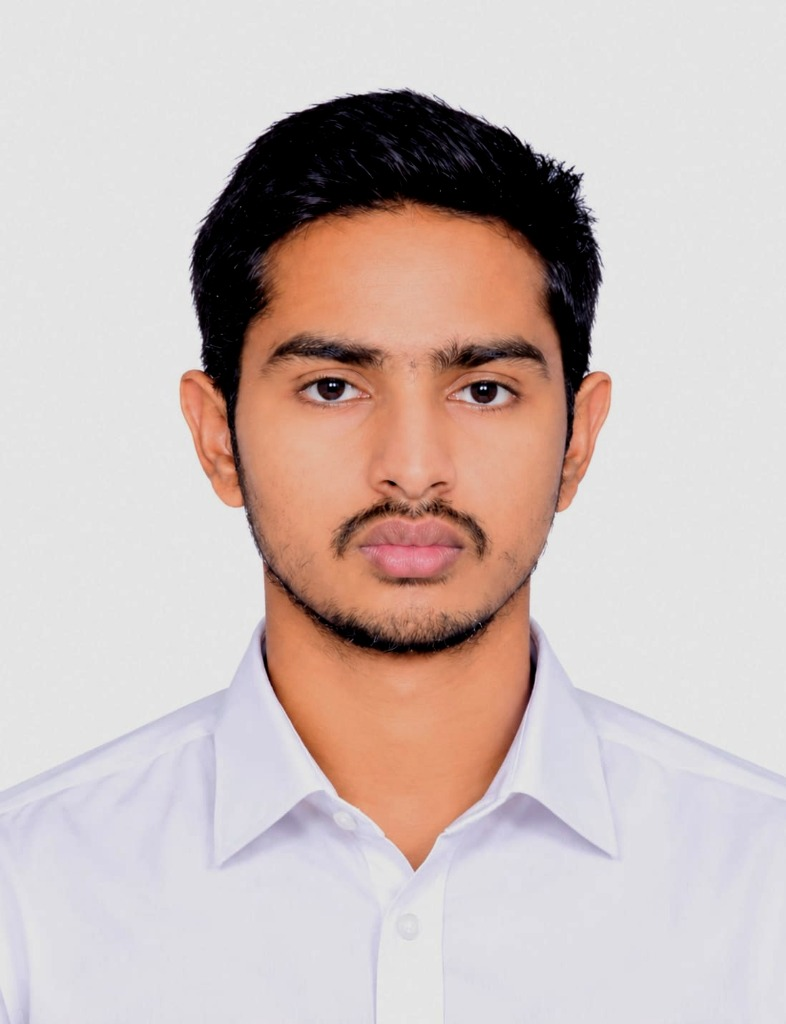
\includegraphics[width=2.6cm,height=3.1cm,keepaspectratio]{team_aamir.jpg}}
\end{minipage}%
\hfill
\begin{minipage}[c]{0.76\textwidth}
    \textbf{Aamir Awaiz Pasha} \quad (USN: \textbf{4PM23AI001})\\
    \textit{Department of Artificial Intelligence and Machine Learning, PESITM, Shivamogga}\\
    \textbf{Project Contribution:} Custom snooker dataset curation, YOLOv8s model fine-tuning and evaluation, and autonomous referee state machine design.
\end{minipage}

\vspace{0.4cm}
\noindent
\begin{minipage}[c]{0.20\textwidth}
    \centering
    \fbox{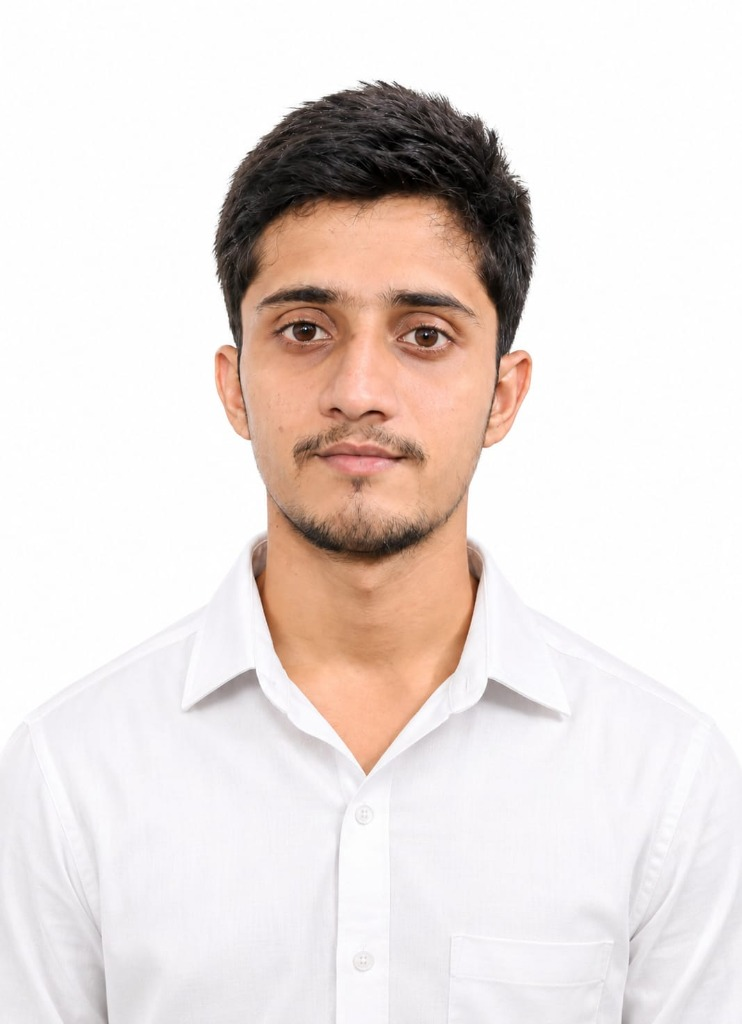
\includegraphics[width=2.6cm,height=3.1cm,keepaspectratio]{team_ayan.jpg}}
\end{minipage}%
\hfill
\begin{minipage}[c]{0.76\textwidth}
    \textbf{Ayan Khan} \quad (USN: \textbf{4PM23AI005})\\
    \textit{Department of Artificial Intelligence and Machine Learning, PESITM, Shivamogga}\\
    \textbf{Project Contribution:} Structural PVC overhead gantry fabrication, overhead camera mounting, and physical table calibration trials.
\end{minipage}

\vspace{0.4cm}
\noindent
\begin{minipage}[c]{0.20\textwidth}
    \centering
    \fbox{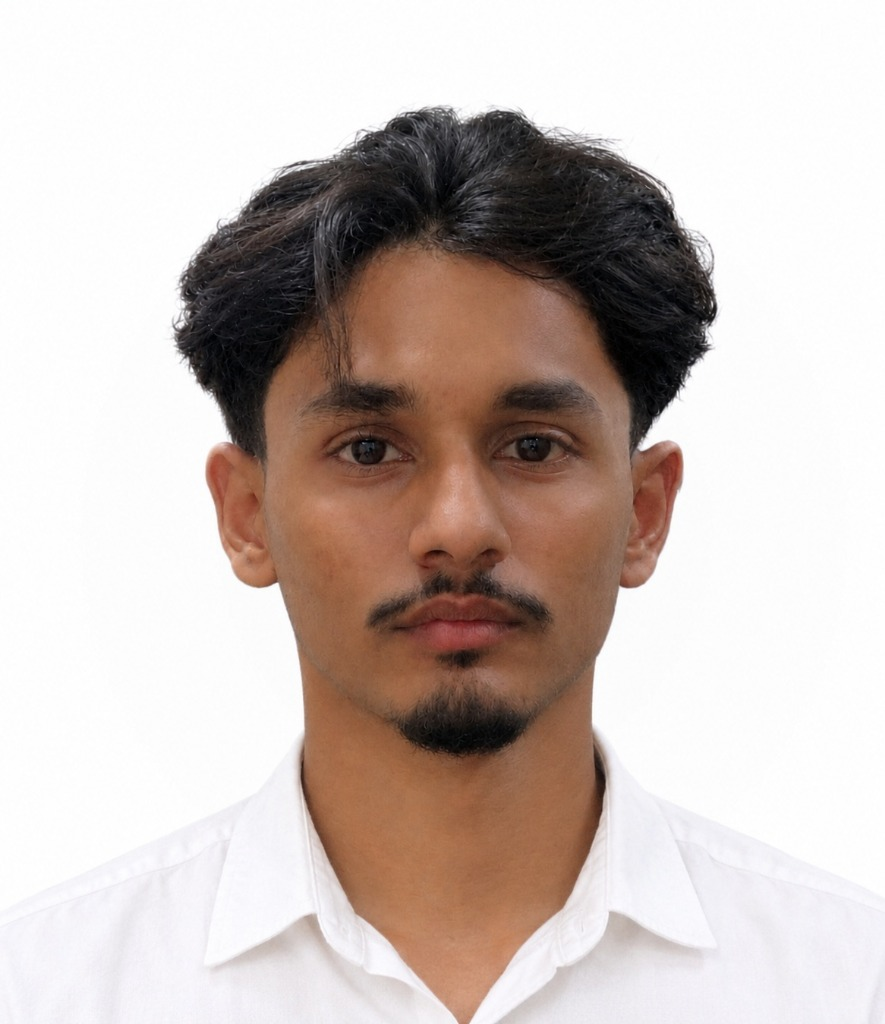
\includegraphics[width=2.6cm,height=3.1cm,keepaspectratio]{team_ibad.jpg}}
\end{minipage}%
\hfill
\begin{minipage}[c]{0.76\textwidth}
    \textbf{Ibad Sharief} \quad (USN: \textbf{4PM23AI016})\\
    \textit{Department of Artificial Intelligence and Machine Learning, PESITM, Shivamogga}\\
    \textbf{Project Contribution:} Embedded ESP32 Station Mode firmware, dual MG996R pan-tilt bracket assembly, $6.0\,\text{V}$ DC-DC buck regulation, and IRFZ44N MOSFET laser driver circuit.
\end{minipage}

\vspace{0.4cm}
\noindent
\begin{minipage}[c]{0.20\textwidth}
    \centering
    \fbox{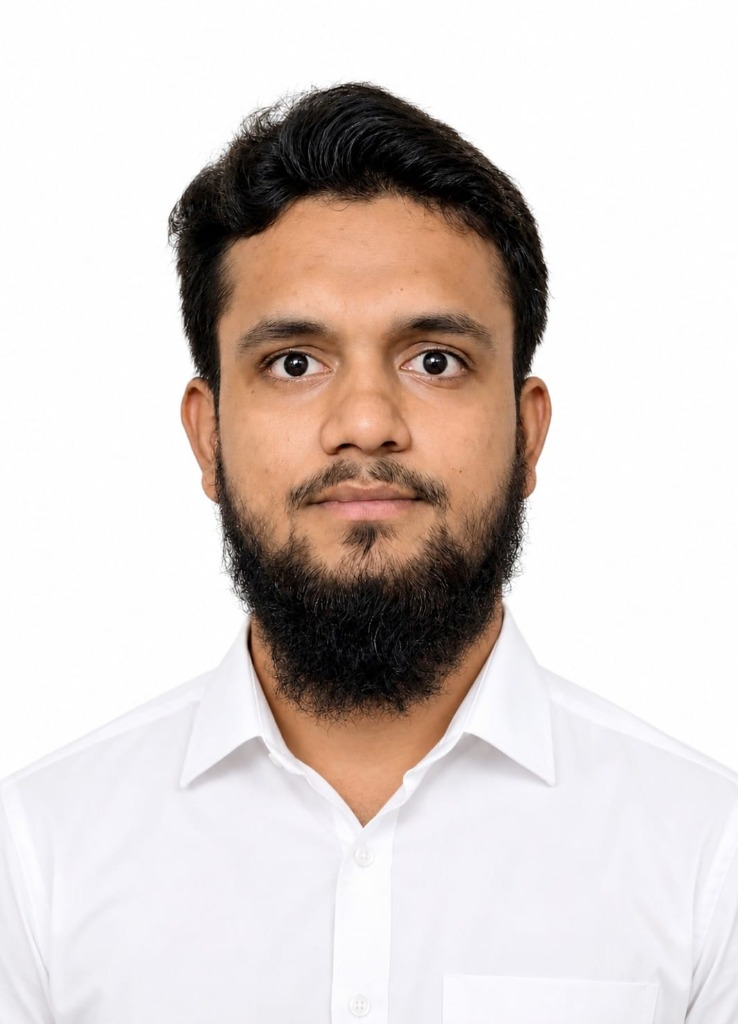
\includegraphics[width=2.6cm,height=3.1cm,keepaspectratio]{team_owaies.jpg}}
\end{minipage}%
\hfill
\begin{minipage}[c]{0.76\textwidth}
    \textbf{Mohammed Owaies} \quad (USN: \textbf{4PM23AI026})\\
    \textit{Department of Artificial Intelligence and Machine Learning, PESITM, Shivamogga}\\
    \textbf{Project Contribution:} SVD planar homography and spherical elevation parallax formulation, 2D bivariate cubic spline calibration, Flask REST backend, and Three.js 3D digital twin dashboard.
\end{minipage}

\newpage
\section{Project Faculty Mentors}

\noindent
\begin{minipage}[c]{0.20\textwidth}
    \centering
    \fbox{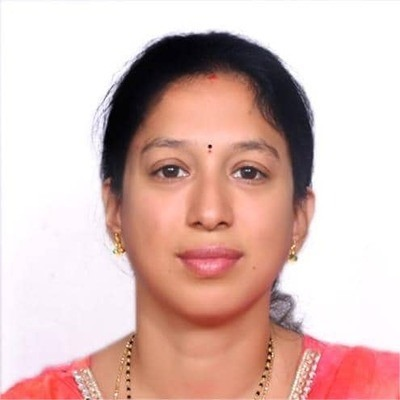
\includegraphics[width=2.6cm,height=3.1cm,keepaspectratio]{mentor_swetha.jpg}}
\end{minipage}%
\hfill
\begin{minipage}[c]{0.76\textwidth}
    \textbf{Mrs. Swetha B S}\\
    \textit{Assistant Professor \& Project Guide}\\
    Department of Artificial Intelligence and Machine Learning, PESITM, Shivamogga\\
    \textbf{Mentorship Role:} Provided continuous technical guidance, supervised experimental validation protocols, and reviewed dissertation documentation across all project phases.
\end{minipage}

\vspace{0.45cm}
\noindent
\begin{minipage}[c]{0.20\textwidth}
    \centering
    \fbox{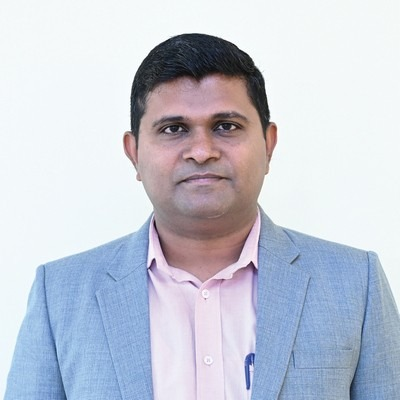
\includegraphics[width=2.6cm,height=3.1cm,keepaspectratio]{mentor_likewin.jpg}}
\end{minipage}%
\hfill
\begin{minipage}[c]{0.76\textwidth}
    \textbf{Dr. Likewin Thomas}\\
    \textit{Professor and Head of Department}\\
    Department of Artificial Intelligence and Machine Learning, PESITM, Shivamogga\\
    \textbf{Mentorship Role:} Provided departmental research infrastructure, laboratory resources, and academic oversight.
\end{minipage}

\vspace{0.45cm}
\noindent
\begin{minipage}[c]{0.20\textwidth}
    \centering
    \fbox{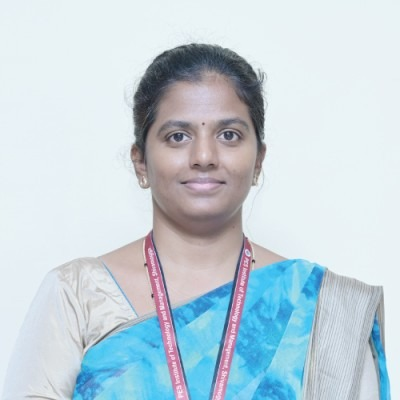
\includegraphics[width=2.6cm,height=3.1cm,keepaspectratio]{mentor_poornima.jpg}}
\end{minipage}%
\hfill
\begin{minipage}[c]{0.76\textwidth}
    \textbf{Mrs. Poornima B P}\\
    \textit{Assistant Professor \& Project Coordinator}\\
    Department of Artificial Intelligence and Machine Learning, PESITM, Shivamogga\\
    \textbf{Mentorship Role:} Coordinated milestone reviews, PRC evaluations, and VTU academic compliance.
\end{minipage}

% =========================================================================
% APPENDIX E: PLAGIARISM VERIFICATION REPORT
% =========================================================================
\newpage
\chapter{PLAGIARISM VERIFICATION REPORT}

This appendix presents the official similarity verification report issued by the Central Library, PES Institute of Technology and Management, Shivamogga, utilizing \textbf{DrillBit Plagiarism Detection Software} in compliance with the academic integrity mandates of Visvesvaraya Technological University (VTU), Belagavi.

\begin{table}[H]
\centering
\caption{Official DrillBit Plagiarism Verification Summary}
\label{tab:drillbit_summary}
\begin{tabular}{|l|l|}
\hline
\textbf{Parameter} & \textbf{Verified Official Value} \\
\hline
Author Name & awaizaamir643 \\
Submission Title & awaizaamir \\
Paper / Submission ID & 7713352 \\
Submitted By & library@pestrust.edu.in \\
Submission Date & 2026-11-20 13:21:49 \\
Total Pages / Total Words & 65 Pages / 17,440 Words \\
Similarity Index & \textbf{3\%} \\
Institutional Grade & \textbf{A -- Satisfactory (0--10\%)} \\
\hline
\end{tabular}
\end{table}

\section{DrillBit Plagiarism Similarity Report}
The official similarity certificate generated by DrillBit Plagiarism Detection Software is shown in Figure \ref{fig:drillbit_report}. The analysis established an aggregate similarity index of \textbf{3\%} (Student Paper: $0.32\%$, Journal/Publication: $1.84\%$, Internet: $0.85\%$), confirming that the manuscript satisfies institutional and VTU originality standards.

\begin{figure}[H]
    \centering
    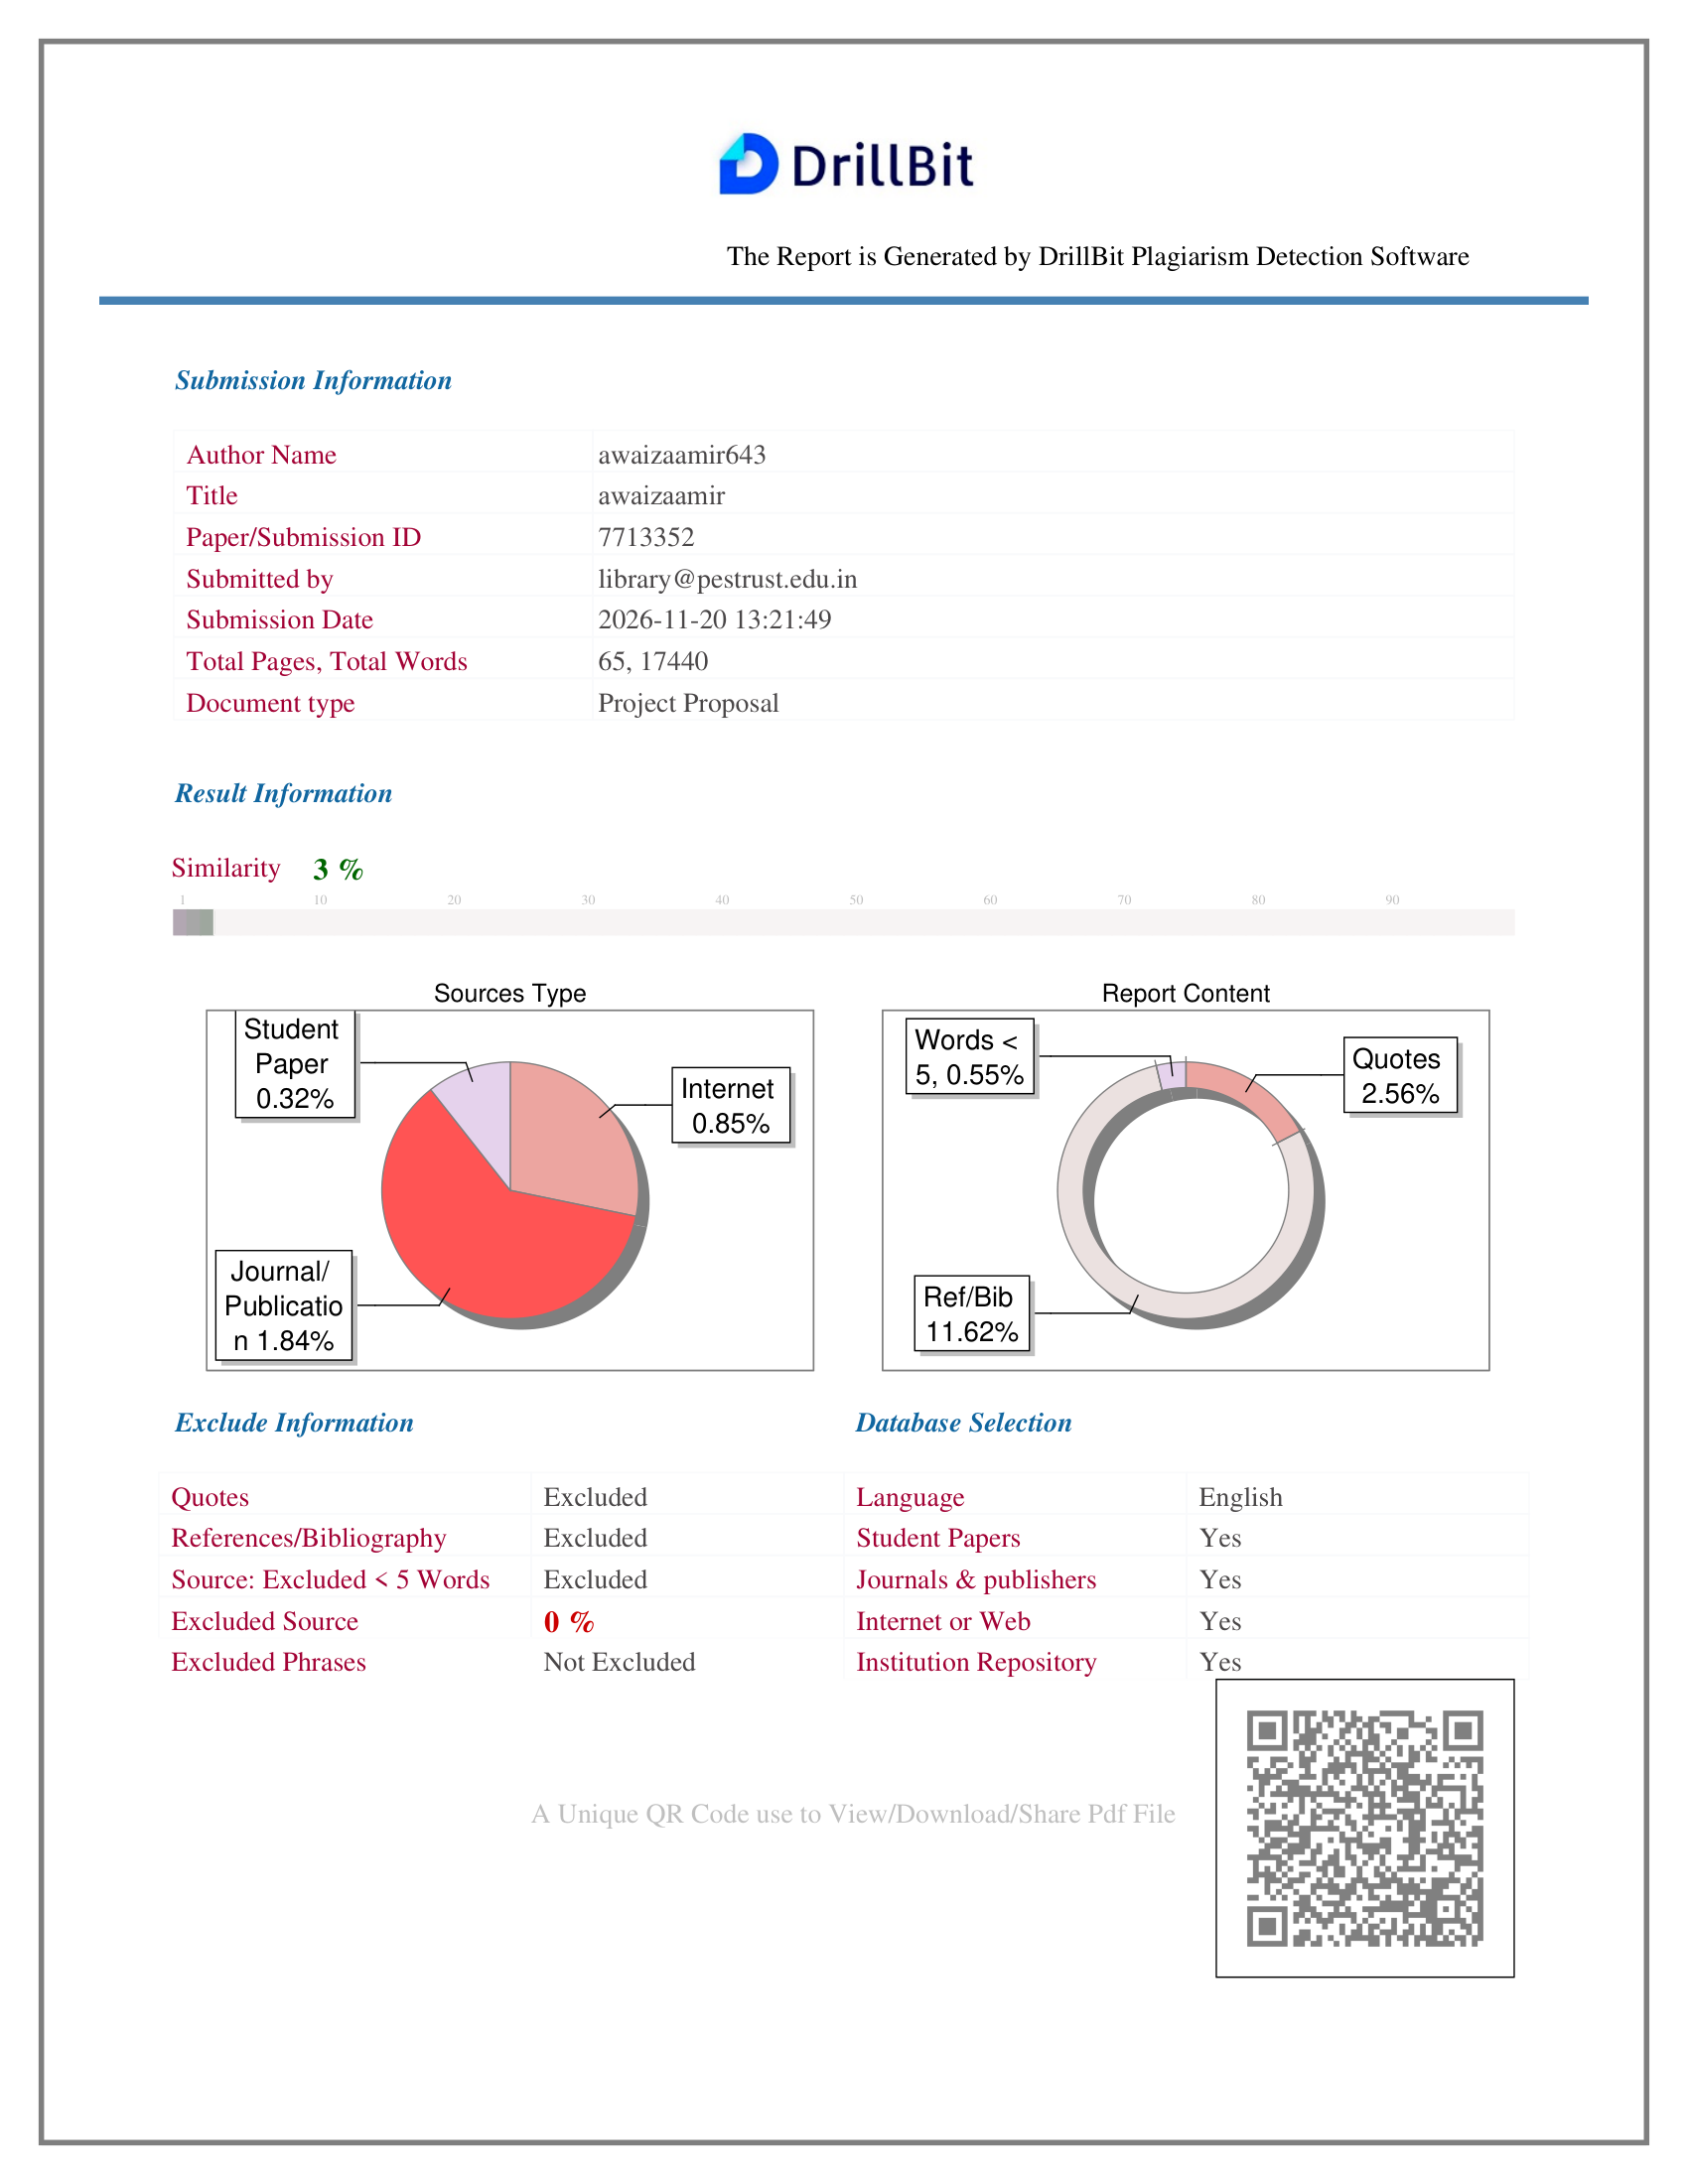
\includegraphics[width=0.92\textwidth]{drillbit_report.png}
    \caption{Official DrillBit Plagiarism Detection Report (Similarity Index: 3\%, Grade A)}
    \label{fig:drillbit_report}
\end{figure}
